\clearpage
\item \subquestionpoints{5}
For Dataset 1, create a plot of the validation set with $x_1$ on the horizontal
axis, and $x_2$ on the vertical axis. To visualize the two classes, use a
different symbol for examples $x^{(i)}$ with $y^{(i)} = 0$ than for those with
$y^{(i)} = 1$. On the same figure, plot the decision boundary found by logistic
regression in part (b). Make an identical plot with the decision boundary found
by GDA in part (e).

\ifnum\solutions=1 {
\begin{answer}\\
\begin{figure}
  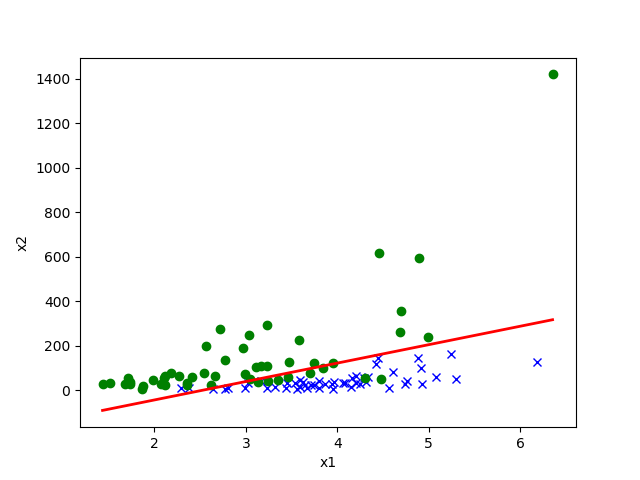
\includegraphics[width=\linewidth]{p01b_pred_1_eval.png}
  \caption{Dateset 1 prediction on EVAL set using LogisticRegression}
  \label{fig:Dateset 1 prediction on EVAL set using LogisticRegression}
\end{figure}\\
\begin{figure}
  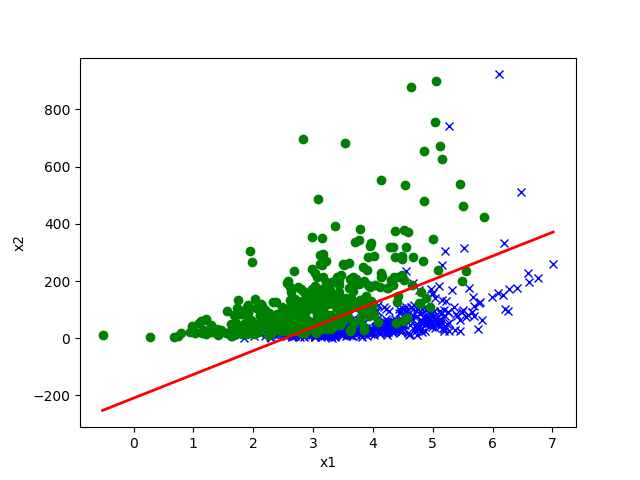
\includegraphics[width=\linewidth]{p01b_pred_1_train.png}
  \caption{Dateset 1 prediction on TRAIN set using LogisticRegression}
  \label{fig:Dateset 1 prediction on TRAIN set using LogisticRegression}
\end{figure}\\
\begin{figure}
  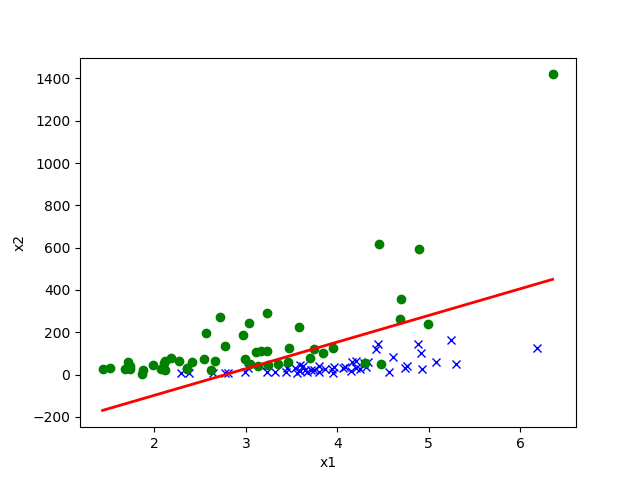
\includegraphics[width=\linewidth]{p01e_pred_1_eval.png}
  \caption{Dateset 1 prediction on EVAL set using GDA}
  \label{fig:Dateset 1 prediction on EVAL set using GDA}
\end{figure}\\
\begin{figure}
  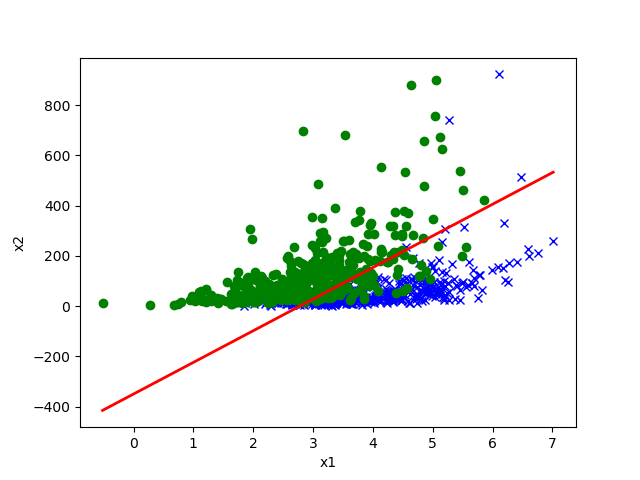
\includegraphics[width=\linewidth]{p01e_pred_1_train.png}
  \caption{Dateset 1 prediction on TRAIN set using GDA}
  \label{fig:Dateset 1 prediction on TRAIN set using GDA}
\end{figure}\\
\end{answer}

} \fi
